\documentclass[10.5pt,scale=1.0,t,aspectratio=169,hyperref={pdfpagelabels=false}]{beamer}
%\usepackage[paperwidth=13.33in, paperheight=7.5in,top=.25in, bottom=.25in, left=.25in, right=.25in]{geometry}
%\geometry{papersize={13.33in,7.5in}}

%\usetheme{Dresden}
%\usetheme{Warsaw}

%Other themes
%https://hartwork.org/beamer-theme-matrix/

\usepackage{lipsum}
\usepackage{color}

\usepackage{amsfonts}
\usepackage{amsmath,mathtools}
\usepackage{mathrsfs}
\usepackage{array}
\usepackage{algorithm}
\usepackage{hyperref}
\usepackage[spanish,es-nodecimaldot]{babel}
\usepackage[utf8]{inputenc}
%\usepackage{intcalc}
\usepackage{graphicx}
\usepackage{multicol}
%\usepackage{authblk}
\usepackage{multirow}
\usepackage{enumitem}
\usepackage[document]{ragged2e}

\usepackage[absolute,overlay]{textpos}
\textblockorigin{0mm}{0mm} 

\usefonttheme[onlymath]{serif}
%\usepackage{epstopdf}
\usepackage{verbatim}
\usepackage{cite}
\usepackage{siunitx}
%\usepackage[texcoord,grid,gridunit=mm,gridcolor=red!10,subgridcolor=green!10]{eso-pic}




\newenvironment{conditions}[1][where:]
  {#1 \begin{tabular}[t]{>{$}l<{$} @{${}={}$} l}}
  {\end{tabular}\\[\belowdisplayskip]}


\newcolumntype{L}{>{$}l<{$}} % math-mode version of "l" column type


\newcounter{saveenumi}
\newcommand{\seti}{\setcounter{saveenumi}{\value{enumi}}}
\newcommand{\conti}{\setcounter{enumi}{\value{saveenumi}}}

\setbeamertemplate{bibliography item}{\insertbiblabel}


\hypersetup{colorlinks=true,
						linkcolor=blue,
						linktoc=all,				
						citecolor=blue,
						urlcolor=red,
						pdftitle={ELECTRONICA DIGITAL II},
						pdfauthor={Santiago Rúa Pérez},
						pdfcreator={Santiago Rúa Pérez}}


\definecolor{GreenDark}{rgb}{0.0, 0.60, 0.0}
\definecolor{RedDark}{rgb}{183, 0.0, 0.0}
\definecolor{BlueDark}{rgb}{0.0, 0.0, 167}
\definecolor{BlueLight}{rgb}{0.2, 0.451, 0.517}


\graphicspath{{imag/}}

\newcommand{\Ho}{$H_{0}$}
\newcommand{\Ha}{$H_{a}$}
\newcommand{\Nota}{{\bf Nota: }}
\newcolumntype{P}[1]{>{\centering\arraybackslash}p{#1}}
\newcolumntype{M}[1]{>{\centering\arraybackslash}m{#1}}

\newcommand{\less}{<}
\newcommand{\greater}{>}


\setlength{\parindent}{1em}
\setlength{\parskip}{.6em}
\renewcommand{\baselinestretch}{.9}

 
\title{Electrónica Digital II}   
\author{Santiago Rúa Pérez, PhD.} 
\date{\today} 

\setlength{\TPHorizModule}{\textwidth}
\setlength{\TPVertModule}{\textwidth}

\newcommand{\btVFill}{\vskip0pt plus 1filll}


\setbeamertemplate{sidebar right}{}
\setbeamertemplate{footline}
{
	\leavevmode%
	\hbox{%
		\begin{beamercolorbox}[wd=.333333\paperwidth,ht=2.25ex,dp=1ex,center]{author in head/foot}%
			\usebeamerfont{author in head/foot}\insertshortauthor
		\end{beamercolorbox}%
		\begin{beamercolorbox}[wd=.333333\paperwidth,ht=2.25ex,dp=1ex,center]{title in head/foot}%
			\usebeamerfont{title in head/foot}\insertshorttitle
	\end{beamercolorbox}}%
	\vskip0pt%
}
\makeatother

\begin{document}
\justify
\renewcommand{\arraystretch}{2.0}


%%%%%%%%%%%%%%%%%% FRAME %%%%%%%%%%%%%%%%%%%%%%%%%%
\begin{frame}
	\titlepage
\end{frame}
%%%%%%%%%%%%%%%%%%% FRAME %%%%%%%%%%%%%%%%%%%%%%%%%%



%%%%%%%%%%%%%%%%% FRAME %%%%%%%%%%%%%%%%%%%%%%%%%%
\begin{frame}
	\frametitle{Objetivos}
{\bf Objetivos}
\begin{itemize}
	\item Definir cantidades análogas y digitales.
	\item Definir ventajas de digital sobre análogo.
	\item Dar ejemplos de digital y análogo.
	\item Definir sistema binario.
	\item Describir las características principales de una señal.
	
\end{itemize}
\end{frame}
%%%%%%%%%%%%%%%%% FRAME %%%%%%%%%%%%%%%%%%%%%%%%%%

%%%%%%%%%%%%%%%%% FRAME %%%%%%%%%%%%%%%%%%%%%%%%%%
\begin{frame}
	\frametitle{Definiciones}
\begin{itemize}
	\item {\bf Análogo}: es una cantidad que tiene valores continuos. 
	\item {\bf Digital}: es una cantidad que tiene uno o varios valores discretos. 
\end{itemize}
\begin{columns}
	\column{0.5\linewidth}
	\begin{block}{\small Análogo}
		\justifying
		\vspace{-0.05in}
		\begin{figure}
			\centering
			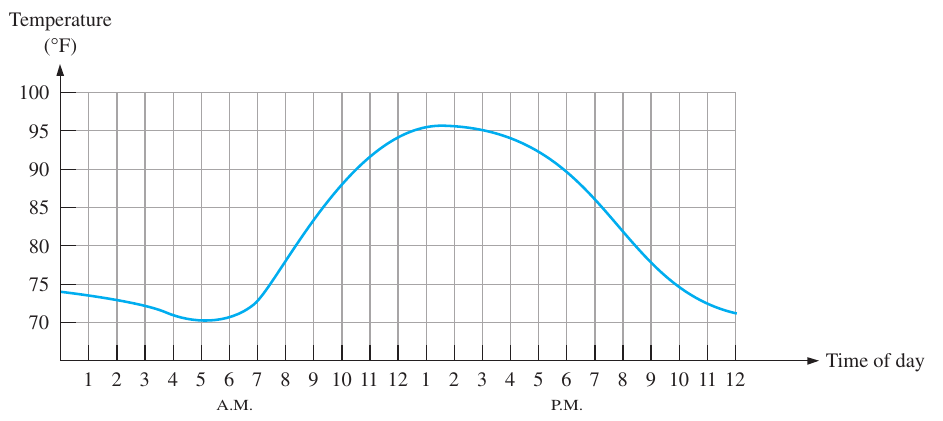
\includegraphics[width=2.1in]{VariableAnaloga}
		\end{figure}
	\end{block}
	
	\column{0.5\linewidth}
	\begin{block}{\small Digital}
		\justifying
		\begin{figure}
			\centering
			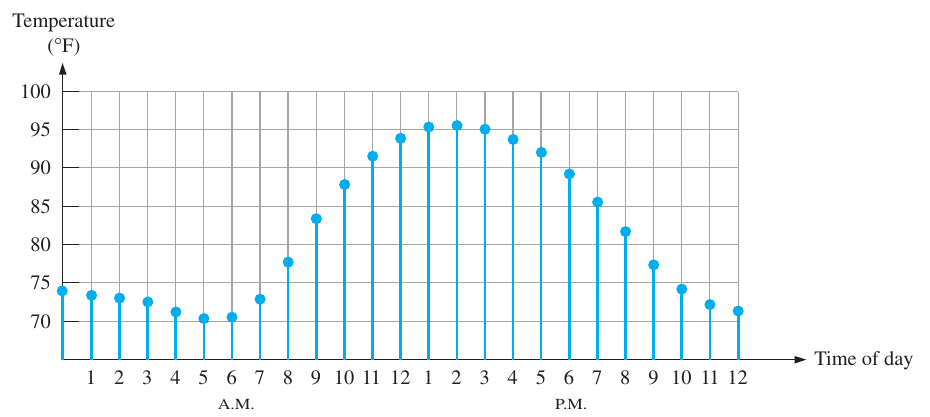
\includegraphics[width=2.1in]{VariableDiscreta}
		\end{figure}
	\end{block}
\end{columns}
\end{frame}
%%%%%%%%%%%%%%%%% FRAME %%%%%%%%%%%%%%%%%%%%%%%%%%
\begin{frame}
\frametitle{Sistema análogo}
 \textcolor{blue}{\large Ejemplo} \\
\begin{figure}
	\centering
	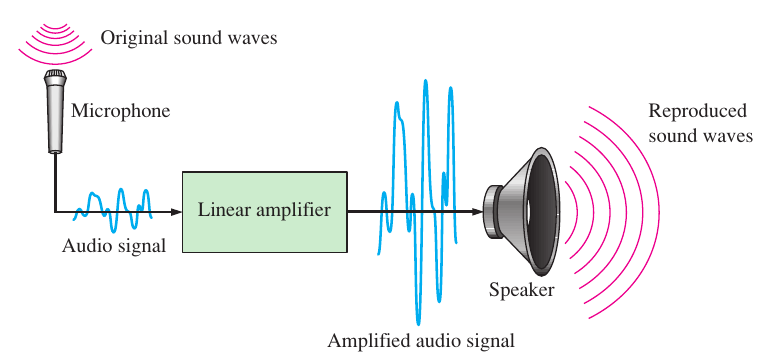
\includegraphics[width=14cm]{SistemaMicrofono}
\end{figure}	
\end{frame}

%%%%%%%%%%%%%%%%% FRAME %%%%%%%%%%%%%%%%%%%%%%%%%%
\begin{frame}
	\frametitle{Sistema digital}
	\textcolor{blue}{\large Ejemplo} \\
\begin{figure}
	\centering
	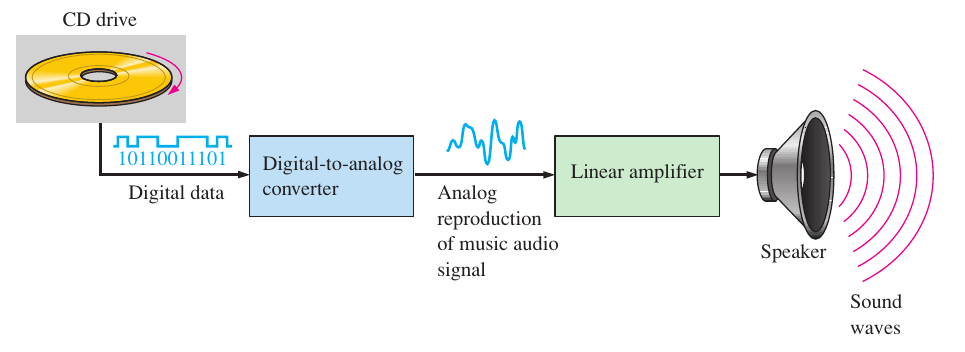
\includegraphics[width=14cm]{SistemaCD}
\end{figure}	
\end{frame}

%%%%%%%%%%%%%%%%% FRAME %%%%%%%%%%%%%%%%%%%%%%%%%%
\begin{frame}
	\frametitle{Mecatrónica}
	\textcolor{blue}{\large Ejemplo} \\
\begin{figure}
	\centering
	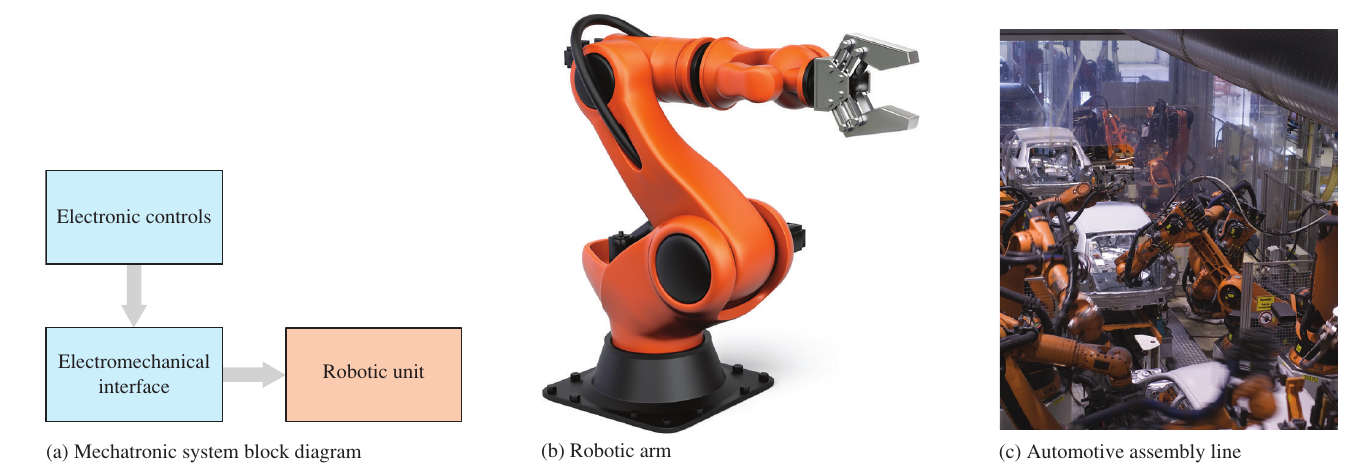
\includegraphics[width=14cm]{Mecatronica}
\end{figure}	
\end{frame}

%%%%%%%%%%%%%%%%% FRAME %%%%%%%%%%%%%%%%%%%%%%%%%%
\begin{frame}
	\frametitle{Digitos Binarios, Niveles y Formas de Onda}
	\justifying
\textcolor{blue}{\large Digitos Binarios} \\
El sistema binario solo cuenta con dos digitos, 0 y 1. En los circuitos digitales dos niveles de voltajes son usados para representar dichos valores. Generalmente 1 representa \textbf{HIGH} y 0 \textbf{LOW}. Lo anterior se conoce como lógica positiva.
\vspace{-0.2in}
\begin{columns}
	\column{0.5\linewidth}
	\begin{block}
		\justifying
		\vspace{-0.3in}
		\begin{figure}
			\centering
			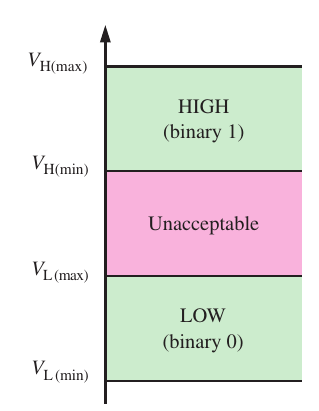
\includegraphics[width=4cm]{RangosNivelesVoltaje}
		\end{figure}
	\end{block}
	
	\column{0.5\linewidth}
	\begin{block}{\small Valores}
		\justifying
		Típicamente para la tecnología CMOS, el nivel de HIGH puede variar entre \SI{2}{\volt} a \SI{3.3}{\volt} y para el LOW entre \SI{0}{\volt} y \SI{0.8}{\volt}.
	\end{block}
\end{columns}	
\end{frame}

%%%%%%%%%%%%%%%%% FRAME %%%%%%%%%%%%%%%%%%%%%%%%%%
\begin{frame}
	\frametitle{Formas de onda digital}
	\vspace{-0.1in}
\begin{figure}
	\centering
	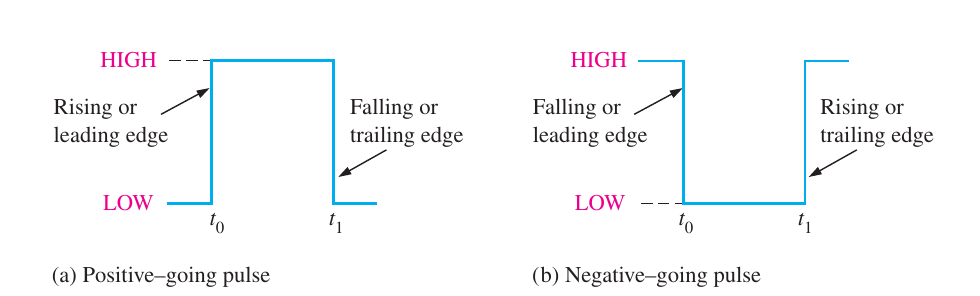
\includegraphics[width=11cm]{FormasOndas}
\end{figure}
\begin{figure}
	\centering
	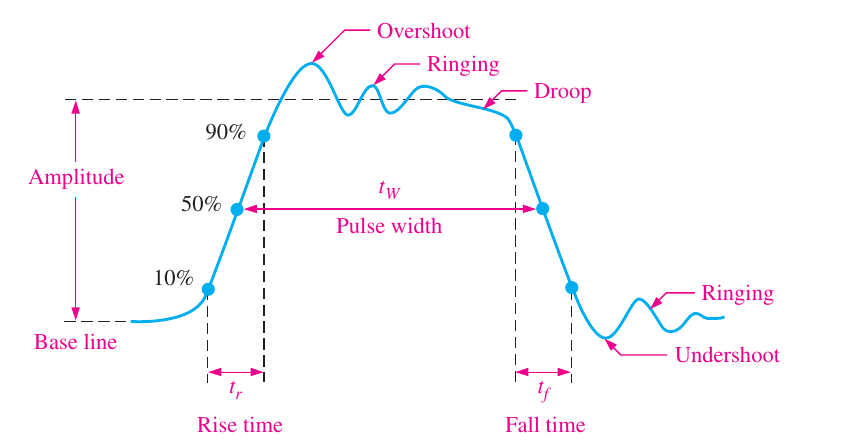
\includegraphics[width=9cm]{PulsoNoIdeal}
\end{figure}	
\end{frame}

%%%%%%%%%%%%%%%%% FRAME %%%%%%%%%%%%%%%%%%%%%%%%%%
\begin{frame}
	\frametitle{Formas de onda}
	\textcolor{blue}{\large Características} \\
\begin{figure}
	\centering
	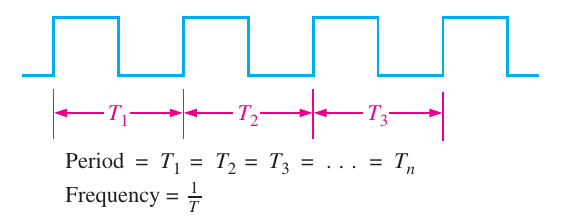
\includegraphics[width=6cm]{PeriodoFrecuencia}
\end{figure}
\textcolor{blue}{\large Clock} \\
\begin{figure}
	\centering
	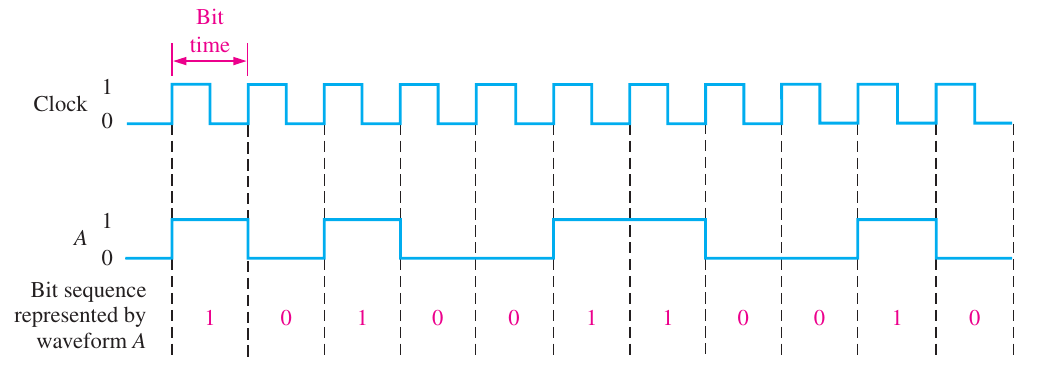
\includegraphics[width=8cm]{Clock}
\end{figure}	
\end{frame}

%%%%%%%%%%%%%%%%% FRAME %%%%%%%%%%%%%%%%%%%%%%%%%%
\begin{frame}
	\frametitle{Formas de onda}
	\textcolor{blue}{\large Ejemplo} \\
En la Figura se muestra una parte de una señal digital periodica. Las medidas estan expresadas en milisegundos. Determinar: frecuencia, periodo y ciclo de trabajo. 
\begin{figure}
	\centering
	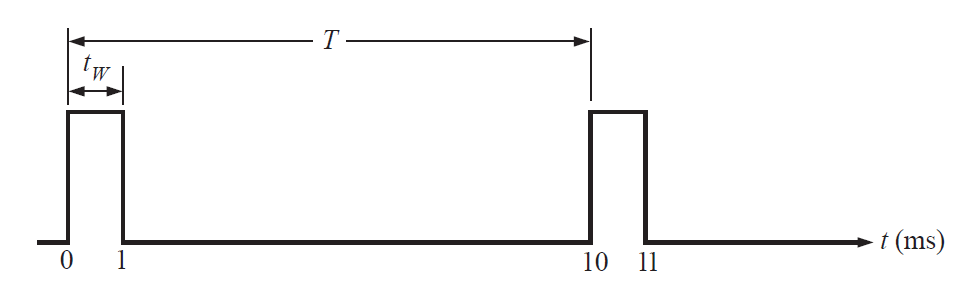
\includegraphics[width=9cm]{EjemploFrecuenciaPeriodo}
\end{figure}	
\end{frame}
%%%%%%%%%%%%%%%%% FRAME %%%%%%%%%%%%%%%%%%%%%%%%%%
\begin{frame}
	\frametitle{Diagramas de tiempo}
	Es una gráfica de señales digitales que muestra la relación temporal real entre dos o más señales y cómo varía cada señal respecto a las demás 
\begin{figure}
	\centering
	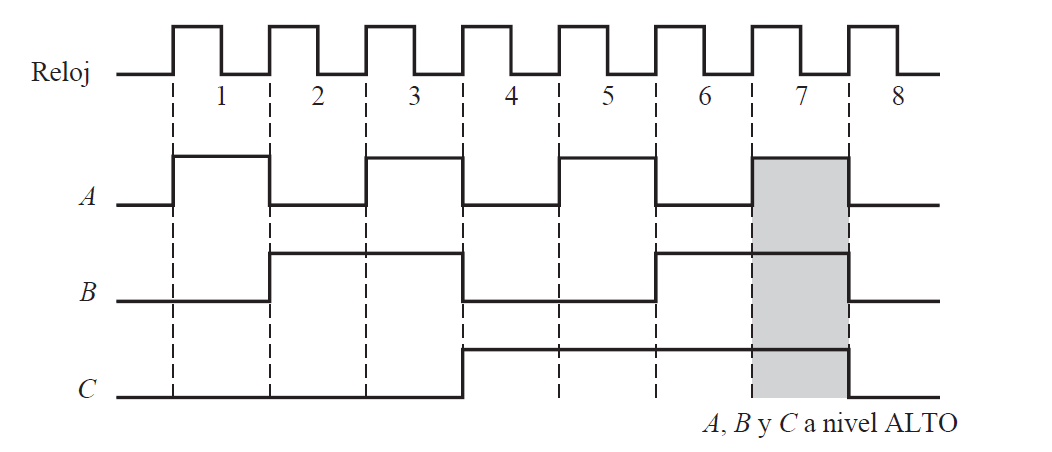
\includegraphics[width=9cm]{DiagramasTiempo}
\end{figure}
\end{frame}

%%%%%%%%%%%%%%%%% FRAME %%%%%%%%%%%%%%%%%%%%%%%%%%
\begin{frame}
	\frametitle{Transferencia de datos}
	\textcolor{blue}{\large Serial} \\
\begin{figure}
	\centering
	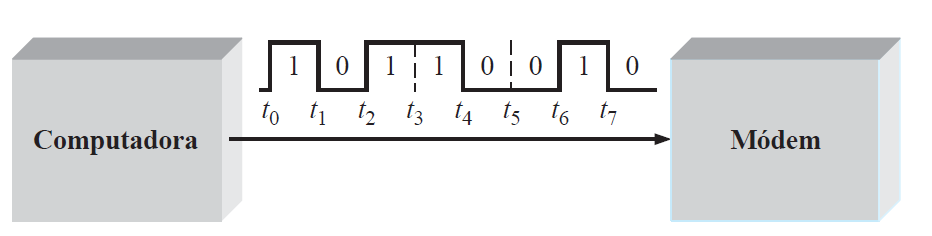
\includegraphics[width=9cm,height=2cm]{TransferenciaSerial}
\end{figure}
\textcolor{blue}{\large Paralela} \\
\begin{figure}
	\centering
	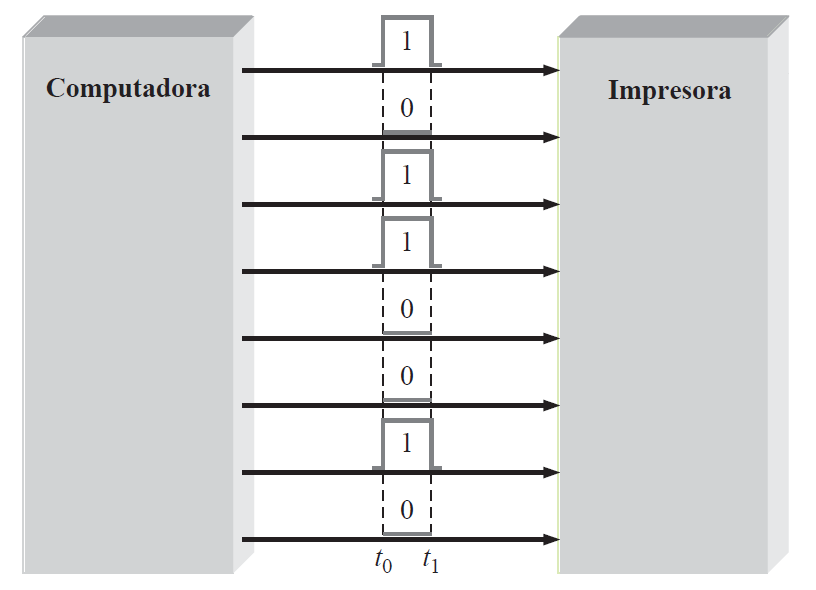
\includegraphics[width=7cm,height=4cm]{TransferenciaParalela}
\end{figure}
\end{frame}

%%%%%%%%%%%%%%%%% FRAME %%%%%%%%%%%%%%%%%%%%%%%%%%
\begin{frame}
	\frametitle{Transferencia de datos}
	\textcolor{blue}{\large Ejemplo} \\
Determinar el tiempo total para transmitir en serie los ocho bits de la señal A mostrada en la Figura. La señal de reloj es de 10 kHz. ¿Cuál es el tiempo para transmitir en paralelo?
\begin{figure}
	\centering
	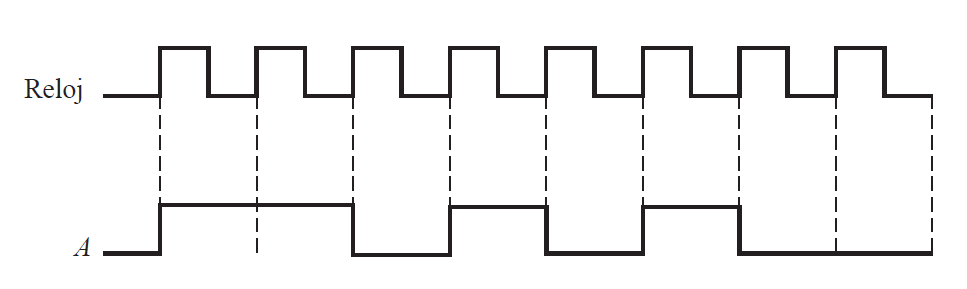
\includegraphics[width=9cm,height=2cm]{EjemploTransferenciaDatos}
\end{figure}
\end{frame}

%%%%%%%%%%%%%%%%% FRAME %%%%%%%%%%%%%%%%%%%%%%%%%%
\begin{frame}
	\frametitle{Operaciones lógicas}
	El término lógico se aplica a los circuitos digitales que se utilizan para implementar funciones lógicas. Existen varios tipos de circuitos lógicos que son los elementos básicos que constituyen los bloques sobre los que se construyen los sistemas digitales más complejos
\begin{figure}
	\centering
	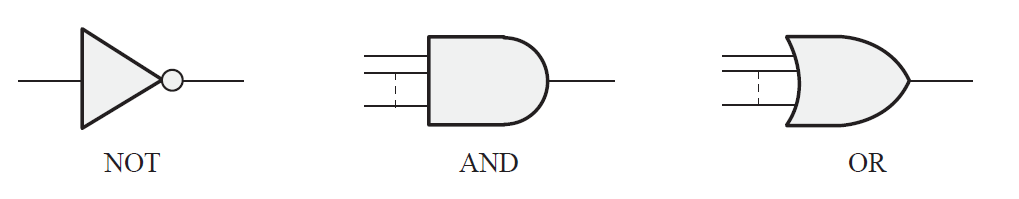
\includegraphics[width=9cm,height=2cm]{CompuertasLogicas}
\end{figure}
\end{frame}

%%%%%%%%%%%%%%%%% FRAME %%%%%%%%%%%%%%%%%%%%%%%%%%
\begin{frame}
	\frametitle{Circuitos integrados}
	Un circuito integrado (CI) monolítico es un circuito electrónico construido enteramente sobre un pequeño chip de silicio. Todos los componentes que conforman el circuito: transistores, diodos, resistencias y condensadores, son parte integrante de un único chip.
\begin{figure}
	\centering
	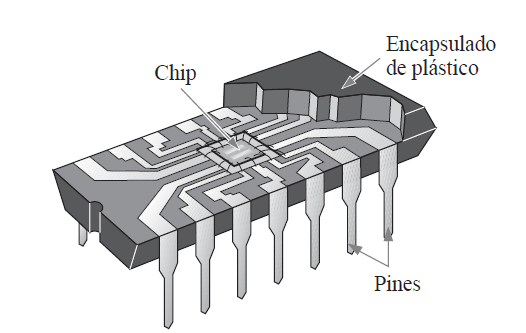
\includegraphics[width=5cm,height=3cm]{CircuitoIntegrado}
\end{figure}
\end{frame}

%%%%%%%%%%%%%%%%% FRAME %%%%%%%%%%%%%%%%%%%%%%%%%%
\begin{frame}
	\frametitle{Encapsulados de los CI}
	Los CI se clasifican de acuerdo a la forma como se ensamblan en los circuitos impresos PCB: inserción o de montaje superficial (SMT)
\begin{figure}
	\centering
	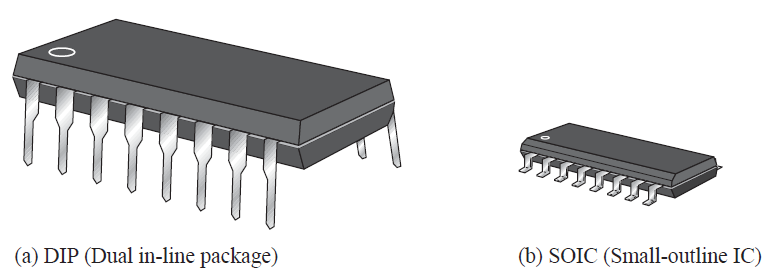
\includegraphics[width=6cm,height=2cm]{TipoIC}
\end{figure}
Los tres tipos de encapsulados SMT más comunes son el SOIC (small-outline IC), el PLCC (plastic leaded chip carrier) y el LCCC (leadless ceramic chip carrier).
\begin{figure}
	\centering
	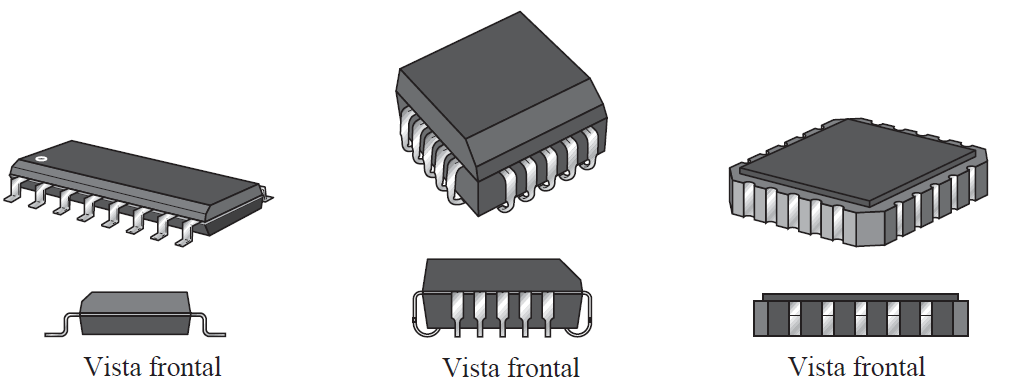
\includegraphics[width=6cm,height=2cm]{SMTClasificacion}
\end{figure}
\end{frame}

%%%%%%%%%%%%%%%%% FRAME %%%%%%%%%%%%%%%%%%%%%%%%%%
\begin{frame}
	\frametitle{Numeración y clasificación de los CI}
	\begin{columns}
	\column{0.5\linewidth}
	\begin{block}
		\justifying
		\vspace{-0.3in}
		\begin{figure}
			\centering
			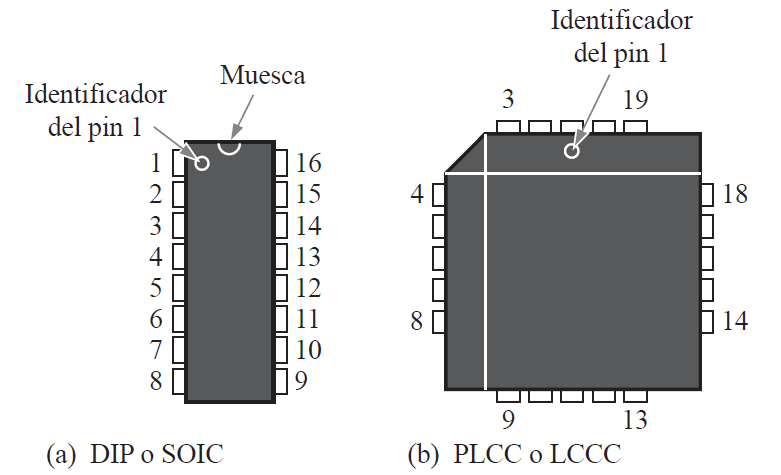
\includegraphics[width=5cm]{NumeracionPines}
		\end{figure}
	\end{block}
	
	\column{0.5\linewidth}
	\begin{block}{\small Clasificación - SI (Scale integration)}
		\justifying
		\small
		\begin{itemize}
			\item SSI: $< 10$ compuertas. Operadores logicos.
			\item MSI: $10 \sim 100$ compuertas. Funciones logicas.
		\end{itemize}
	\end{block}
\end{columns}
\begin{itemize}
	\item LSI: $100 \sim 10000$ Chips, memorias.
	\item VLSI: $10000 \sim 100000$ Chips con funciones especiales
	\item ULSI:$>100000$ Microprocesadores.
\end{itemize}
\end{frame}


%%%%%%%%%%%%%%%%% FRAME %%%%%%%%%%%%%%%%%%%%%%%%%%
\begin{frame}
	\frametitle{Introducción a las funciones lógicas básicas}
		\begin{columns}
	\column{0.5\linewidth}
	\begin{block}{\small Comparación}
		\justifying
		\vspace{-0.1in}
		\begin{figure}
			\centering
			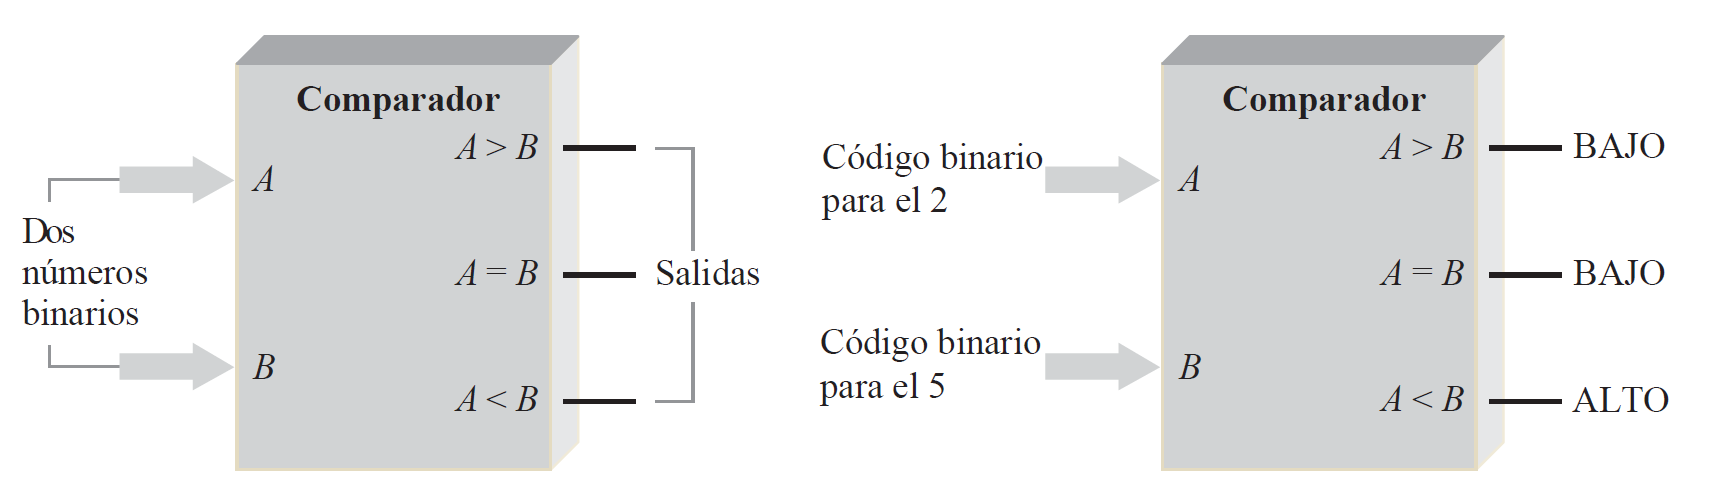
\includegraphics[width=6cm]{FuncionComparador}
		\end{figure}
	\end{block}
	
	\begin{block}{\small Aritmeticas}
		\justifying
		\vspace{-0.1in}
		\begin{figure}
			\centering
			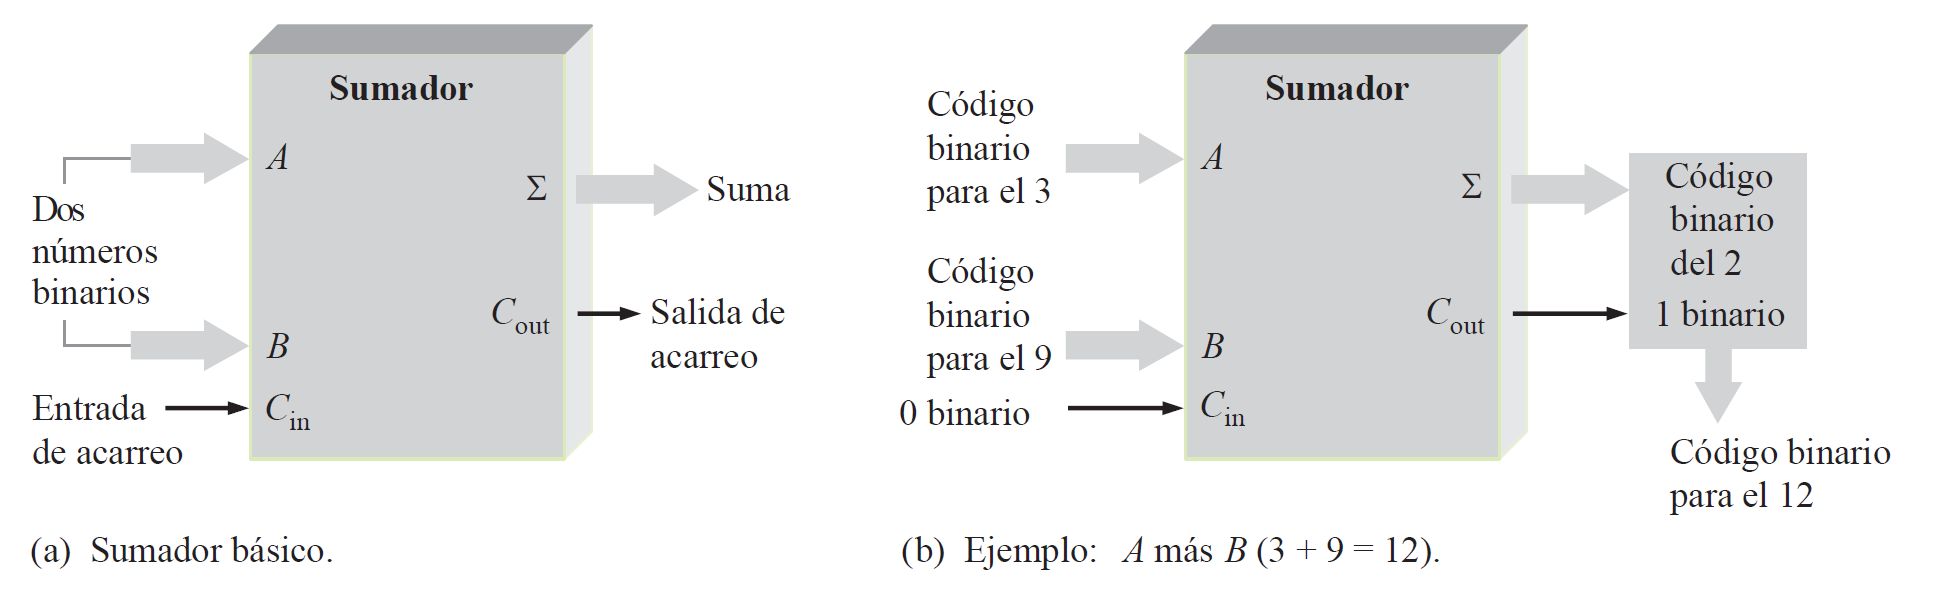
\includegraphics[width=6cm]{FuncionSuma}
		\end{figure}
	\end{block}
	
	%%% Columna 2
	
	\column{0.5\linewidth}
	\begin{block}{\small Codificador}
		\justifying
		\vspace{-0.1in}
		\begin{figure}
			\centering
			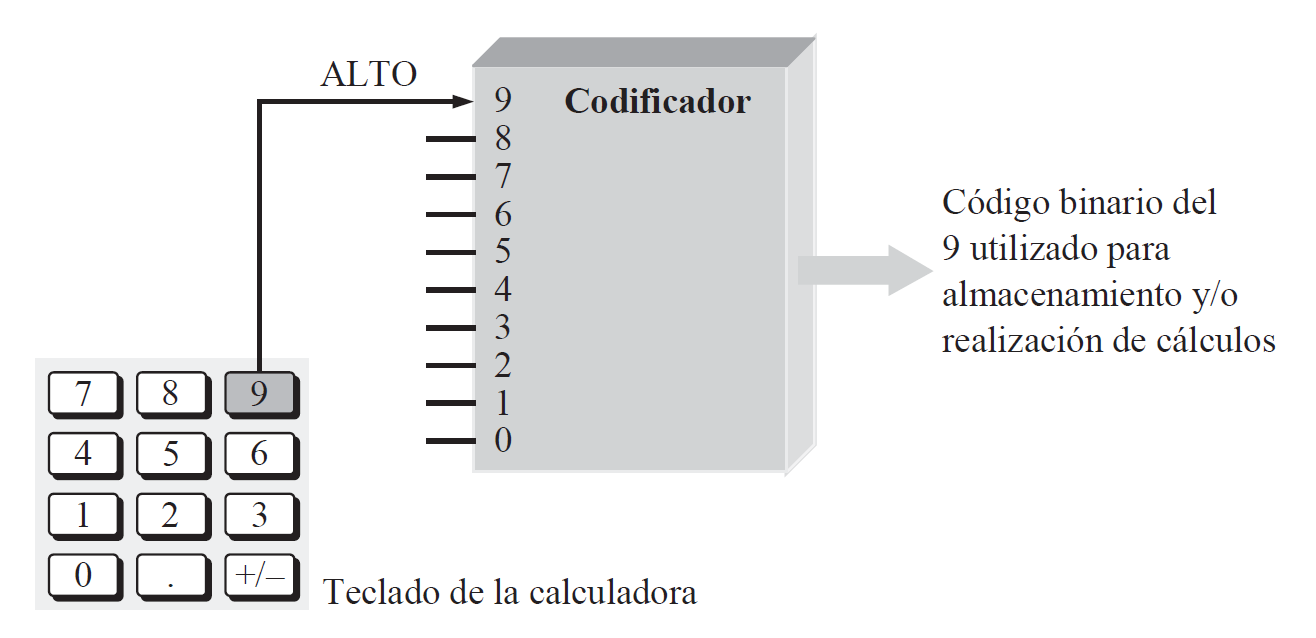
\includegraphics[width=5cm]{FuncionCodificador}
		\end{figure}
	\end{block}
	
	\begin{block}{\small Decodificador}
		\justifying
		\vspace{-0.1in}
		\begin{figure}
			\centering
			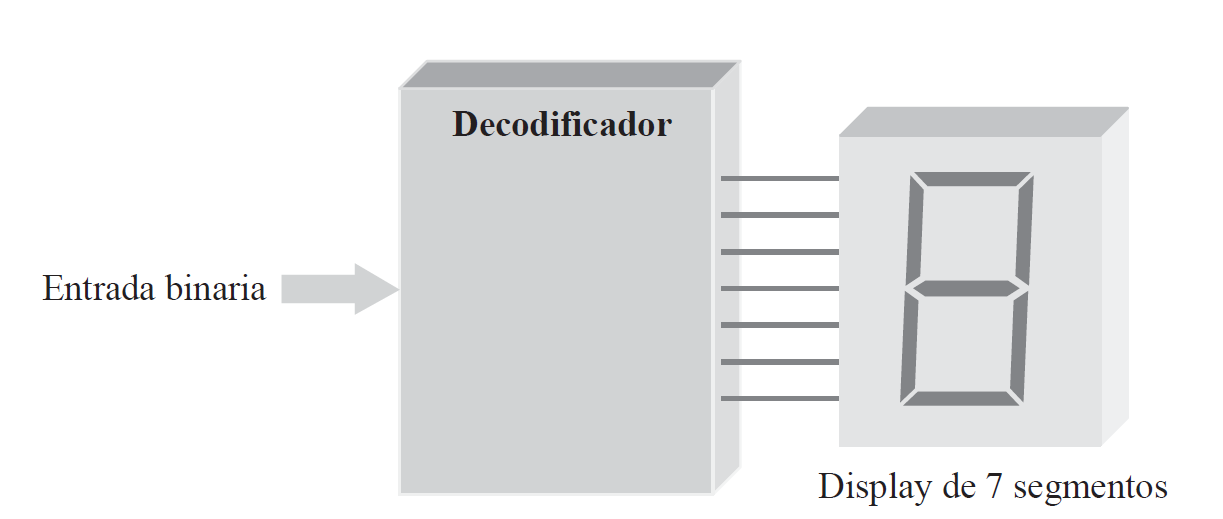
\includegraphics[width=5cm]{FuncionDecodificador}
		\end{figure}
	\end{block}
\end{columns}
\end{frame}


%%%%%%%%%%%%%%%%% FRAME %%%%%%%%%%%%%%%%%%%%%%%%%%
\begin{frame}
	\frametitle{Introducción a las funciones lógicas básicas}
		\begin{block}{\small Multiplexador y Demultiplexador}
	\justifying
	\vspace{-0.1in}
	\begin{figure}
		\centering
		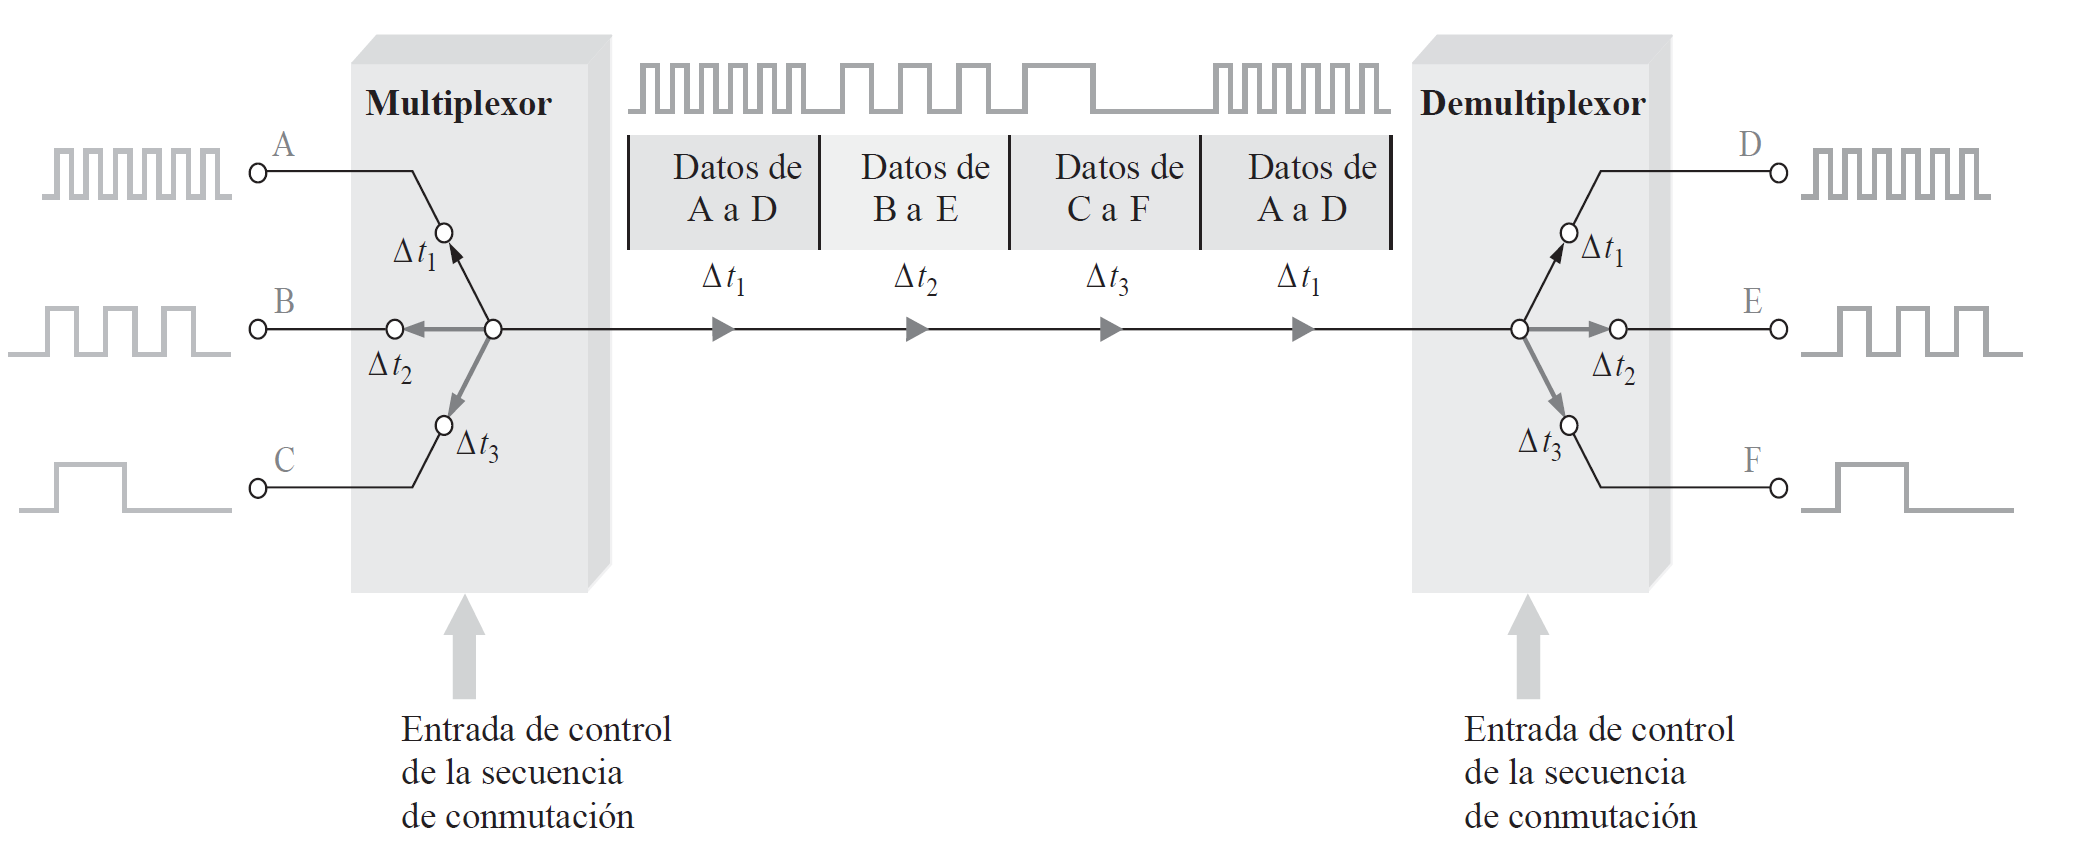
\includegraphics[width=10cm]{MultiplexadorAndDemultiplexador}
	\end{figure}
\end{block}

\begin{block}{\small Contadores}
	\justifying
	\vspace{-0.1in}
	\begin{figure}
		\centering
		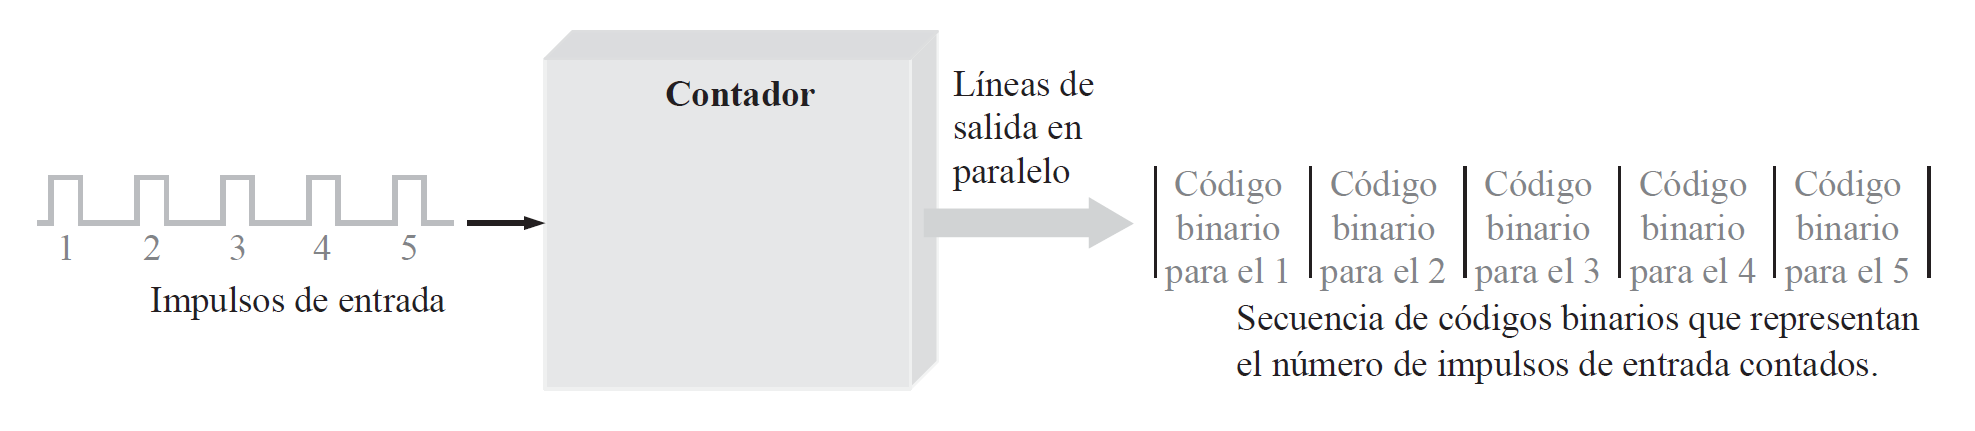
\includegraphics[width=10cm]{Contadores}
	\end{figure}
\end{block}
\end{frame}

%%%%%%%%%%%%%%%%% FRAME %%%%%%%%%%%%%%%%%%%%%%%%%%
\begin{frame}
	\frametitle{Ejemplo sistema digital}
	\vspace{-0.1in}
\begin{figure}
	\centering
	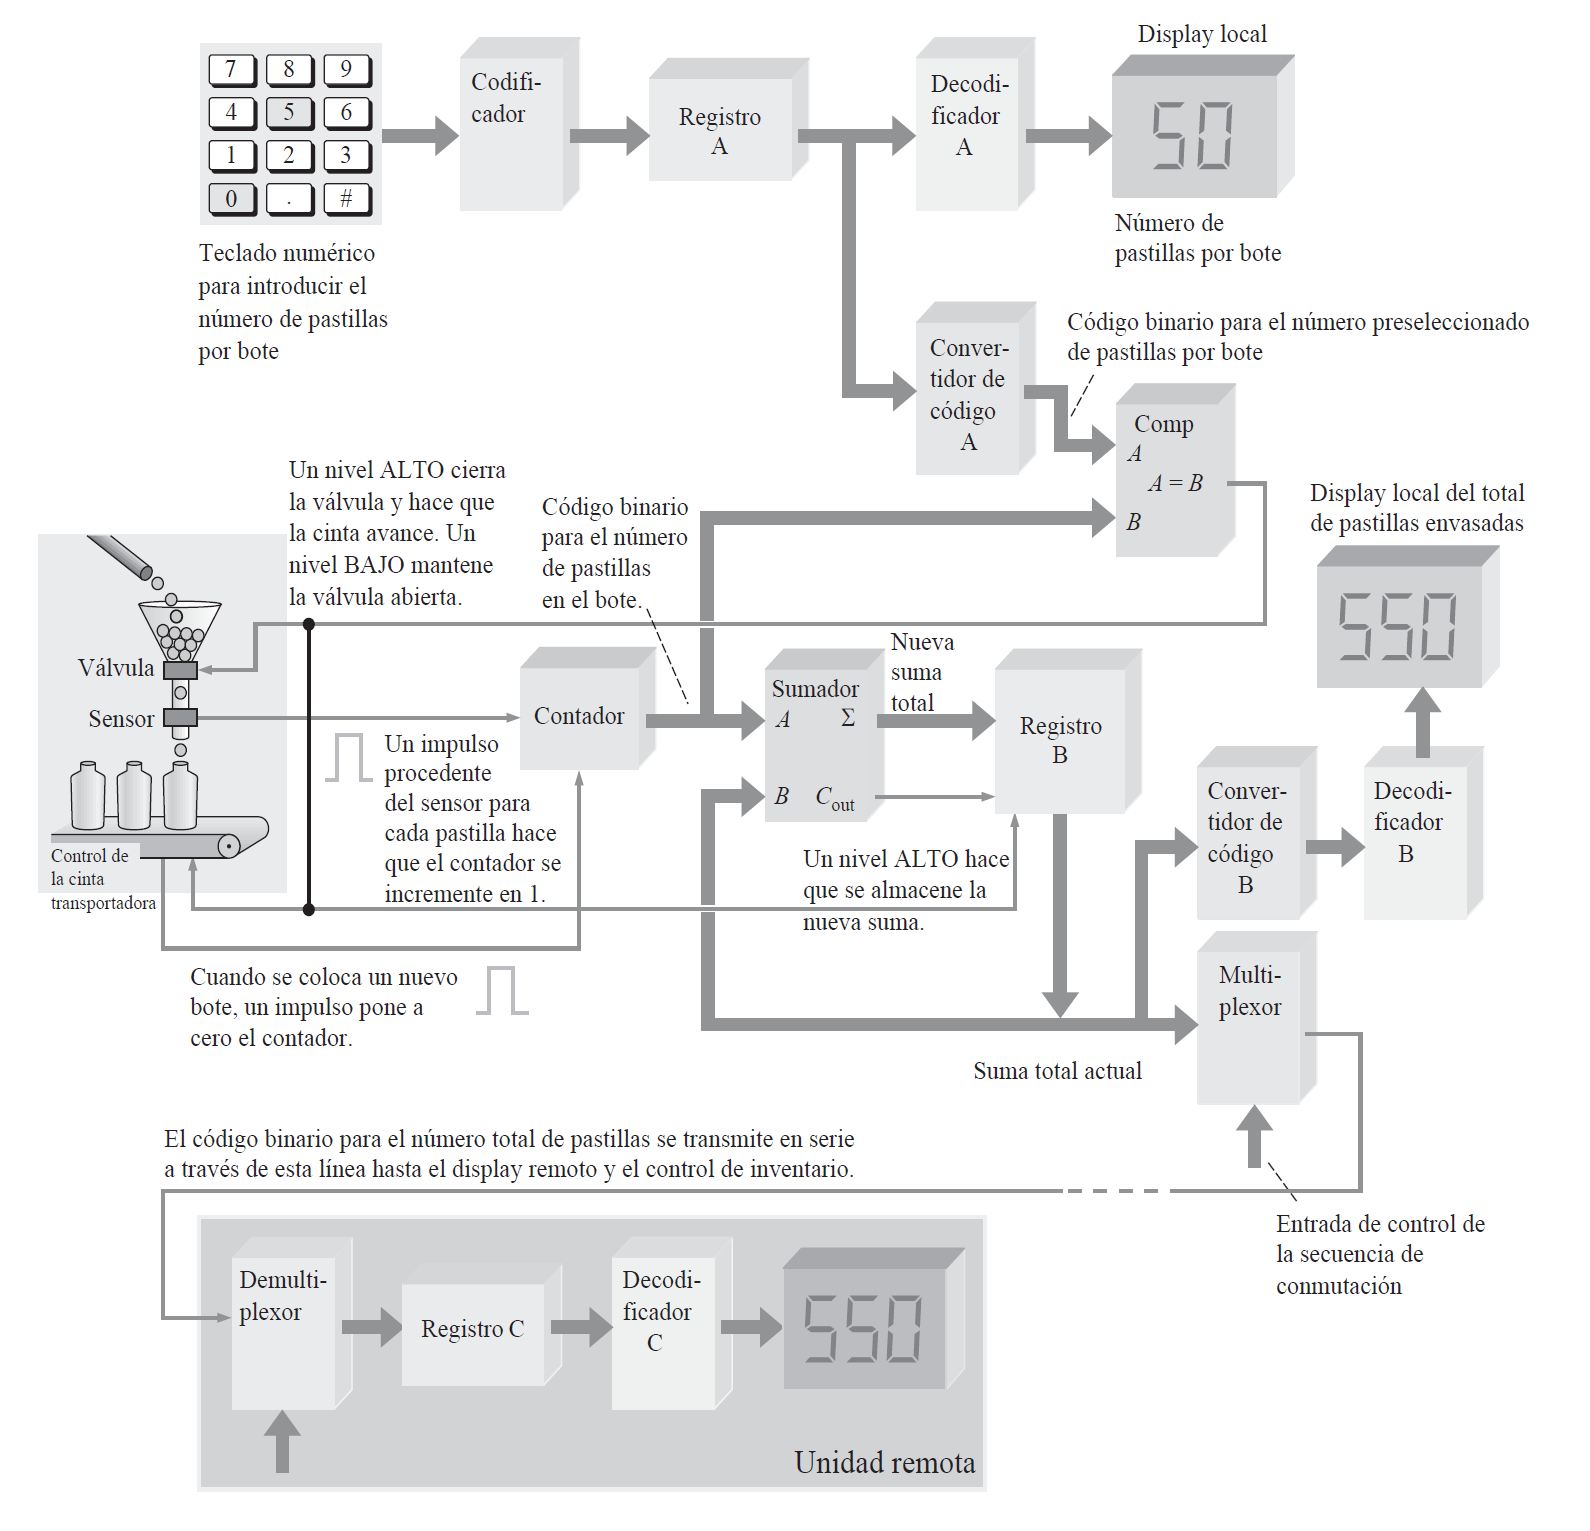
\includegraphics[width=9cm]{EjemploSistemaDigital}
\end{figure}
\end{frame}

%%%%%%%%%%%%%%%%% FRAME %%%%%%%%%%%%%%%%%%%%%%%%%%
\begin{frame}
	\frametitle{Introducción a la lógica programable}
	\vspace{-0.1in}
\begin{figure}
	\centering
	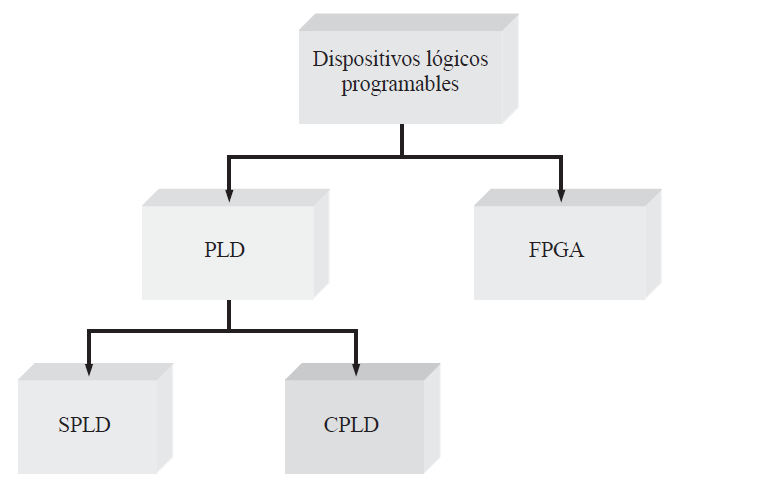
\includegraphics[scale=0.5]{LogicaProgramable}
\end{figure}
PLD (Programmable Logic Device) : dispositivo logico programable.
FPGA (Field Programmable Gate Array): matrices de compuertas programables por campo. 
\end{frame}

%%%%%%%%%%%%%%%%% FRAME %%%%%%%%%%%%%%%%%%%%%%%%%%
\begin{frame}
	\frametitle{Introducción a la lógica programable}
	\vspace{-0.1in}
\textcolor{blue}{\large Simple Programmable Logic Device (SPLD)} \\
\begin{itemize}
	\item Disponible para escalas bajas (pocas compuertas).
	\item Puede reemplazar de 1 a 10 circuitos integrados.
	\item Se clasifican en: PAL (programmable array logic) y GAL (generic array logic).
\end{itemize}
\begin{figure}
	\centering
	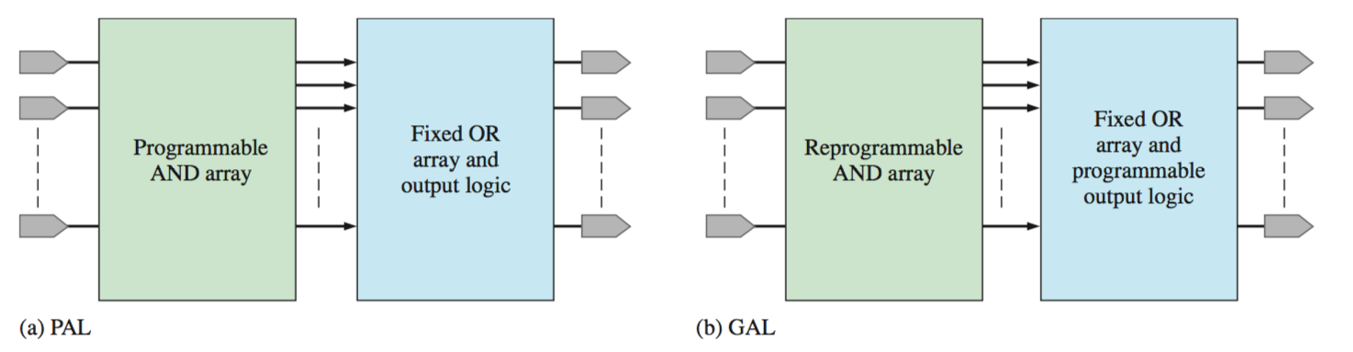
\includegraphics[scale=0.5]{PAL_GAL}
\end{figure}
\end{frame}

%%%%%%%%%%%%%%%%% FRAME %%%%%%%%%%%%%%%%%%%%%%%%%%
\begin{frame}
	\frametitle{Introducción a la lógica programable}
	\vspace{-0.1in}
\textcolor{blue}{\large Complex Programmable Logic Device (CPLD)} \\
\begin{itemize}
	\item Varios SPLD en un solo chip.
	\item Puede reemplazar varios circuitos integrados.
	\item Está compuesto por bloques lógicos (LAB) e interconexiones  de arreglos programables (PIA).
\end{itemize}
\begin{figure}
	\centering
	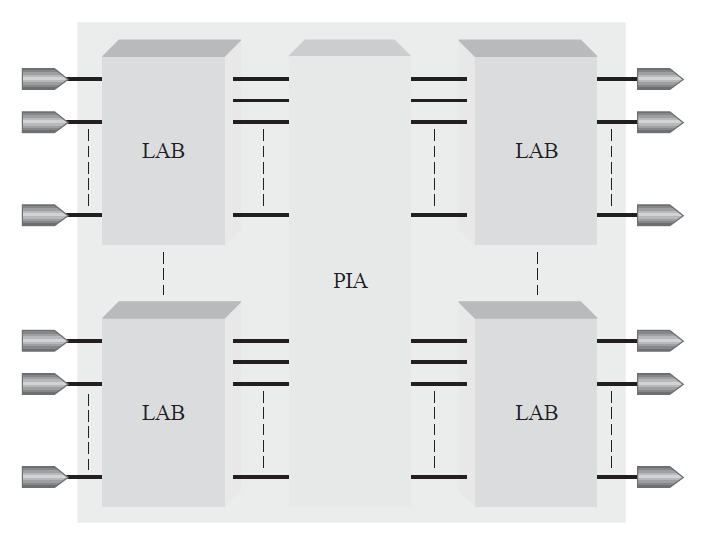
\includegraphics[scale=0.5]{CPLD}
\end{figure}
\end{frame}

%%%%%%%%%%%%%%%%% FRAME %%%%%%%%%%%%%%%%%%%%%%%%%%
\begin{frame}
	\frametitle{Introducción a la lógica programable}
	\vspace{-0.1in}
\textcolor{blue}{\large Field Programmable Gate Array (FPGA)} \\
La estructura de la FPGA (matriz de compuertas programables) es diferente en que se basa en tres elementos: bloques lógicos, bloques de I/O, e interconexiones programables.
\begin{figure}
	\centering
	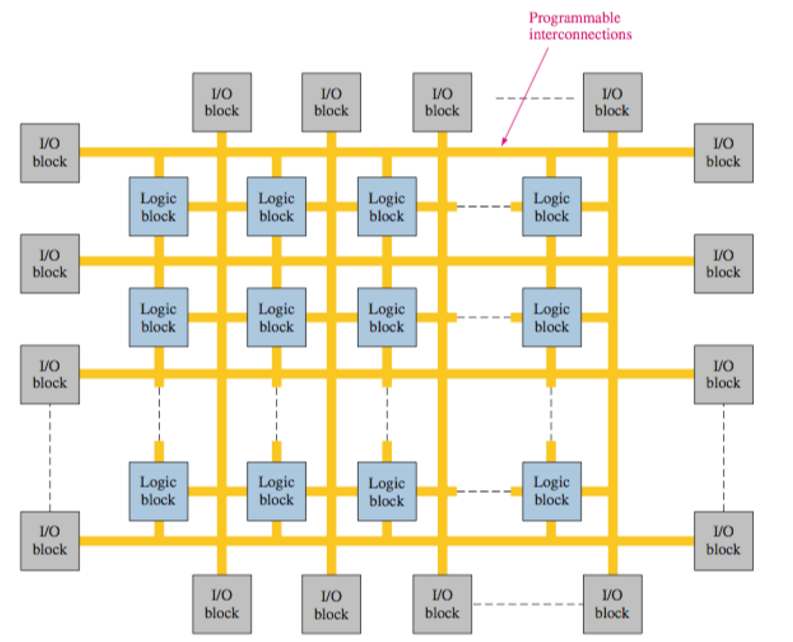
\includegraphics[scale=0.5]{FPGA}
\end{figure} 
\end{frame}

%%%%%%%%%%%%%%%%% FRAME %%%%%%%%%%%%%%%%%%%%%%%%%%
\begin{frame}
	\frametitle{Bibliografia}
	\begin{itemize}
		\item Floyd, T.(2006). \textit{Fundamentos de sistemas digitales}. Pearson Education, 9 edicion, pp 1024.
		\item Tocci, R.J., Widmer, N.S., and Moss, G.L. (2007). Sistemas digitales, principios y aplicaciones. Pearson Education, decima edición, pp 970. 
	\end{itemize} 
\end{frame}
%%%%%%%%%%%%%%%%%% FRAME %%%%%%%%%%%%%%%%%%%%%%%%%%
%\begin{frame}[allowframebreaks]
%\frametitle{BIBLIOGRAFÍA}
%%\nocite{*}
%\bibliographystyle{IEEEtran}
%\bibliography{ReferenceEDE}
%\end{frame}
%%%%%%%%%%%%%%%%%% FRAME %%%%%%%%%%%%%%%%%%%%%%%%%%

\end{document}

